\vspace{2mm}
\ffigbox[\FBwidth]{%
\caption{\centering Ensemble de graphes}\label{fig:dm1_ex05_f2}
}{
    \fbox{

    \begin{subfigure}{68.68655pt}
    \centering
    \fbox{
    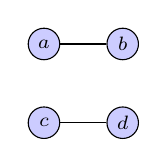
\begin{tikzpicture}[scale=1, main node/.style={circle, draw, fill=blue!20, inner sep=1pt, font=\scriptsize, minimum size=4mm, text=black}]
        \node[main node] (1) at (0,0) {\(a\)};
        \node[main node] (2) at (1,0) {\(b\)};
        \node[main node] (3) at (0,-1) {\(c\)};
        \node[main node] (4) at (1,-1) {\(d\)};
        \draw (1) -- (2);
        \draw (3) -- (4);
    \end{tikzpicture}
    }
    \caption{Un couplage}\label{fig:dm1_ex05_f2_sub1} 
    \end{subfigure}

    \begin{subfigure}{68.68655pt}
    \centering
    \fbox{
    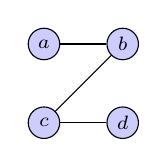
\begin{tikzpicture}[scale=1, main node/.style={circle, draw, fill=blue!20, inner sep=1pt, font=\scriptsize, minimum size=4mm, text=black}]
        \node[main node] (1) at (0,0) {\(a\)};
        \node[main node] (2) at (1,0) {\(b\)};
        \node[main node] (3) at (0,-1) {\(c\)};
        \node[main node] (4) at (1,-1) {\(d\)};
        \draw (1) -- (2);
        \draw (2) -- (3);
        \draw (3) -- (4);
    \end{tikzpicture}
    }
    \caption{Un chemin}\label{fig:dm1_ex05_f2_sub2} % chktex 10
    \end{subfigure}

    \begin{subfigure}{94.58174pt}
    \centering
    \fbox{
    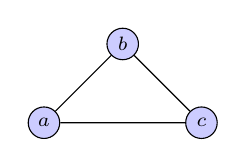
\begin{tikzpicture}[scale=1, main node/.style={circle, draw, fill=blue!20, inner sep=1pt, font=\scriptsize, minimum size=4mm, text=black}]
        \node[main node] (1) at (0,0) {\(a\)};
        \node[main node] (2) at (1,1) {\(b\)};
        \node[main node] (3) at (2,0) {\(c\)};
        \draw (1) -- (2) -- (3) -- (1);
    \end{tikzpicture}
    }
    \caption{Un triangle}\label{fig:dm1_ex05_f2_sub3} % chktex 10
    \end{subfigure}
    }
    
} % chktex 10 chktex 17